\chapter{化学动力学：速率方程}\label{ch:b1:rate-laws}

牛奶放在冰箱里可以保存一周，放在夏天的桌上却只能保存一天。
药品包装盒上写着“请保存在 \qty{25}{\celsius} 以下”，并印有
两三年之后的有效期，厂家来不及直接观察。
平衡常数说明反应进行到何处为止，
却不能说明到达那里需要多长时间。这正是
化学动力学的研究范围。本章定义\omterm{def:b1:rate-laws:rate}{反应速率}，
给出用浓度表示的\omterm{def:b1:rate-laws:order}{速率方程}、能预测任意时刻浓度的积分形式、
介绍确定\omterm{def:b1:rate-laws:order}{速率方程}的实验方法，
以及描述温度影响的\omterm{thm:b1:rate-laws:arrhenius}{阿伦尼乌斯定律}——
正是借助它，只需几周的实验，便可预测
药品的货架寿命。

\begin{recall}
第 1 册（十二年级）介绍了物质的\omterm{def:b1:rate-laws:rate}{生成速率}与\omterm{def:b1:rate-laws:rate}{消耗速率}，
动力学因素（浓度、温度、催化剂）以及
一级反应的\omterm{def:b1:rate-laws:half-life}{半衰期}。\omterm{def:b1:extent-q-and-k:extent}{反应进度} $\xi$ 的定义
见\cref{def:b1:extent-q-and-k:extent}。
\end{recall}

\begin{omfigure}

\includegraphics[width=0.55\linewidth]{images/book2/ai/b1-08-milk-kitchen.jpg}

{\small 一瓶牛奶放在阳光下，紧挨着敞开的冰箱。
使牛奶变质的反应在夏季温度下
比在低温时快好几倍。}
\end{omfigure}

\section{反应速率}

\begin{definition}[反应速率、生成速率与消耗速率]\label{def:b1:rate-laws:rate}
对于反应 $0 = \sum_i \nu_i\mathrm{A}_i$，
设其在体积为 $V$ 的恒容密闭反应器中进行，则称\emph{反应速率}\index{反应速率}
为
\[
  v = \frac{1}{V}\frac{\dd\xi}{\dd t} = \frac{1}{\nu_i}\frac{\dd[\mathrm{A}_i]}{\dd t}
  \quad\text{（对任意 } i\text{）},
\]
其单位为 \unit{mol.L^{-1}.s^{-1}}。产物的\emph{生成速率}\index{生成速率}为
$\dd[\mathrm{A}_i]/\dd t$；反应物的
\emph{消耗速率}\index{消耗速率}为
$-\dd[\mathrm{A}_i]/\dd t$。
\end{definition}

\begin{proposition}[各物质速率一致]\label{prop:b1:rate-laws:rate-relations}
\omterm{def:b1:rate-laws:rate}{反应速率}与选用哪种物质来跟踪无关：
对于 $a\,\mathrm{A} + b\,\mathrm{B} \longrightarrow c\,\mathrm{C} + d\,\mathrm{D}$，
\[
  v = -\frac1a\frac{\dd[\ce{A}]}{\dd t} = -\frac1b\frac{\dd[\ce{B}]}{\dd t}
  = \frac1c\frac{\dd[\ce{C}]}{\dd t} = \frac1d\frac{\dd[\ce{D}]}{\dd t} .
\]
\end{proposition}

\begin{proof}
$[\mathrm{A}_i] = (n_{i,0} + \nu_i\xi)/V$，其中 $V$ 为常数，故
$\dd[\mathrm{A}_i]/\dd t = (\nu_i/V)\,\dd\xi/\dd t = \nu_i v$。
\end{proof}

\begin{example}[五氧化二氮的分解]\label{ex:b1:rate-laws:n2o5}
对于 \ce{2N2O5 -> 4NO2 + O2}：$v = -\frac12\frac{\dd[\ce{N2O5}]}{\dd t} =
\frac14\frac{\dd[\ce{NO2}]}{\dd t} = \frac{\dd[\ce{O2}]}{\dd t}$。二氧化氮
的\omterm{def:b1:rate-laws:rate}{生成速率}是氧气的四倍，五氧化二氮的
\omterm{def:b1:rate-laws:rate}{消耗速率}是氧气\omterm{def:b1:rate-laws:rate}{生成速率}的两倍。
\end{example}

\section{速率方程与级数}

\begin{definition}[速率方程、级数、速率常数]\label{def:b1:rate-laws:order}
\emph{速率方程}\index{速率方程}把速率表示为浓度的函数。
若某反应的速率方程取
如下形式，则称该反应\emph{具有级数}：
\[
  v = k\,[\mathrm{A}]^{p}\,[\mathrm{B}]^{q} \cdots ;
\]
指数 $p$、$q$、\dots\ 称为
对 A、B、\dots\ 的\emph{分级数}\index{分级数}，它们之和称为
\emph{总级数}\index{总级数}，$k$ 称为\emph{速率常数}\index{速率常数}，
它只依赖于温度。级数由
实验确定；它们不必等于\omterm{def:b1:extent-q-and-k:extent}{化学计量数}，并且
可以是分数或零。
\end{definition}

\begin{remark}[$k$ 的单位]\label{rem:b1:rate-laws:units}
由于 $v$ 的单位为 \unit{mol.L^{-1}.s^{-1}}，故 $k$ 的单位
在零级时为 \unit{mol.L^{-1}.s^{-1}}，一级时为 \unit{s^{-1}}，
二级时为 \unit{L.mol^{-1}.s^{-1}}，
一般地为 $(\unit{mol/L})^{1-n}\,\unit{s^{-1}}$，其中\omterm{def:b1:rate-laws:order}{总级数}为 $n$。
$k$ 的单位说明了\omterm{def:b1:rate-laws:order}{总级数}。
\end{remark}

\begin{remark}[无级数的反应]\label{rem:b1:rate-laws:no-order}
并非所有反应都有级数。某些反应的速率是一个分式，
其分母含有浓度，或者依赖于
产物的浓度。这类\omterm{def:b1:rate-laws:order}{速率方程}需要用
反应机理来解释（见\cref{ch:b1:elementary-steps}）。
反应还可能只在起始阶段具有级数，称为初始\omterm{def:b1:rate-laws:order}{速率方程}。
\end{remark}

\section{积分速率方程与半衰期}

\begin{definition}[半衰期]\label{def:b1:rate-laws:half-life}
反应物的\emph{半衰期}\index{半衰期} $t_{1/2}$ 是指
其初始量被消耗一半所需的时间。
\end{definition}

\begin{theorem}[积分速率方程]\label{thm:b1:rate-laws:integrated}
对于反应 $a\mathrm{A} \rightarrow \text{产物}$，速率为 $v = -\frac1a\frac{\dd[\ce{A}]}
{\dd t} = k[\ce{A}]^n$，设 $[\ce{A}](0) = a_0$：
\begin{center}
\begin{tabular}{llll}
\hline
级数 & 积分式 & 线性作图 & \omterm{def:b1:rate-laws:half-life}{半衰期} \\
\hline
0 & $[\ce{A}] = a_0 - akt$ & $[\ce{A}]$ 对 $t$ 作图 & $a_0/(2ak)$ \\
1 & $[\ce{A}] = a_0\,\eu^{-akt}$ & $\ln[\ce{A}]$ 对 $t$ 作图 & $\ln2/(ak)$ \\
2 & $\dfrac{1}{[\ce{A}]} = \dfrac{1}{a_0} + akt$ & $1/[\ce{A}]$ 对 $t$ 作图 & $1/(ak\,a_0)$ \\
\hline
\end{tabular}
\end{center}
\end{theorem}

\begin{proof}
记 $c = [\ce{A}]$，则 $\dd c/\dd t = -akc^n$。
\emph{零级}：$\dd c/\dd t = -ak$，于是 $c = a_0 - akt$（在
$c = 0$ 之前成立）。\emph{一级}：$\dd c/\dd t = -akc$ 是一阶线性
微分方程，其解为 $c = a_0\eu^{-akt}$。
\emph{二级}：$\dd c/c^2 = -ak\,\dd t$；积分，自 0 到 $t$，
$-1/c + 1/a_0 = -akt$，于是 $1/c = 1/a_0 + akt$。\omterm{def:b1:rate-laws:half-life}{半衰期}：令 $c =
a_0/2$，在各定律中解出 $t$。
\end{proof}

\begin{proposition}[半衰期检验]\label{prop:b1:rate-laws:half-life-test}
\omterm{def:b1:rate-laws:half-life}{半衰期}与初始浓度无关，当且仅当
反应为一级。零级时\omterm{def:b1:rate-laws:half-life}{半衰期}正比于 $a_0$，
二级时正比于 $1/a_0$。一级反应每次损失剩余量的一半，
在每个相继的\omterm{def:b1:rate-laws:half-life}{半衰期}内减半：经过 $m$ 个\omterm{def:b1:rate-laws:half-life}{半衰期}后，
剩余分数为 $2^{-m}$。
\end{proposition}

\begin{proof}
对于 $n \ne 1$ 的级数，分离变量可得 $t_{1/2} = \dfrac{2^{n-1} -
1}{(n-1)\,ak\,a_0^{n-1}}$，依赖于 $a_0$，除非 $n = 1$；当
$n = 1$ 时，$t_{1/2} = \ln2/(ak)$。对一级，$c(t + t_{1/2}) = c(t)/2$
在每个 $t$ 处，因为 $\eu^{-ak(t + t_{1/2})} = \eu^{-akt}/2$。
\end{proof}

\begin{omfigure}
\begin{tikzpicture}
\begin{axis}[name=p0,
  width=0.36\linewidth, height=4.6cm,
  xmin=0, xmax=60, ymin=0, ymax=1.05,
  axis x line=bottom, axis y line=left,
  xlabel={$t$ (min)}, title={零级：$[\ce{A}]$},
  title style={font=\small}, xtick={0,20,40,60},
  tick label style={font=\scriptsize}, label style={font=\small}]
\addplot[omDef, thick] table[x=t, y=A0] {figdata/out/bachelor-1-integrated-rate-laws.dat};
\end{axis}
\begin{axis}[at={(p0.east)}, anchor=west, xshift=0.9cm, name=p1,
  width=0.36\linewidth, height=4.6cm,
  xmin=0, xmax=60, ymin=-3.2, ymax=0.2,
  axis x line=bottom, axis y line=left,
  xlabel={$t$ (min)}, title={一级：$\ln[\ce{A}]$},
  title style={font=\small}, xtick={0,20,40,60},
  tick label style={font=\scriptsize}, label style={font=\small}]
\addplot[omProp, thick] table[x=t, y=lnA1] {figdata/out/bachelor-1-integrated-rate-laws.dat};
\end{axis}
\begin{axis}[at={(p1.east)}, anchor=west, xshift=0.9cm,
  width=0.36\linewidth, height=4.6cm,
  xmin=0, xmax=60, ymin=0, ymax=4.2,
  axis x line=bottom, axis y line=left,
  xlabel={$t$ (min)}, title={二级：$1/[\ce{A}]$},
  title style={font=\small}, xtick={0,20,40,60},
  tick label style={font=\scriptsize}, label style={font=\small}]
\addplot[omThm, thick] table[x=t, y=invA2] {figdata/out/bachelor-1-integrated-rate-laws.dat};
\end{axis}
\end{tikzpicture}

\begin{tikzpicture}
\begin{axis}[
  width=0.62\linewidth, height=5.0cm,
  xmin=0, xmax=60, ymin=0, ymax=1.05,
  axis x line=bottom, axis y line=left,
  xlabel={$t$ (min)}, ylabel={$[\ce{A}]$ (mol/L)}, xtick={0,10,20,30,40,50,60},
  tick label style={font=\small}, label style={font=\small},
  legend style={font=\small, draw=none, at={(0.98,0.98)}, anchor=north east}]
\addplot[omDef, thick] table[x=t, y=A0] {figdata/out/bachelor-1-integrated-rate-laws.dat};
\addplot[omProp, thick] table[x=t, y=A1] {figdata/out/bachelor-1-integrated-rate-laws.dat};
\addplot[omThm, thick] table[x=t, y=A2] {figdata/out/bachelor-1-integrated-rate-laws.dat};
\legend{零级, 一级, 二级}
\draw[dotted] (axis cs:0,0.5) -- (axis cs:20,0.5);
\end{axis}
\end{tikzpicture}

{\small 三个反应具有相同的初始浓度
（\qty{1.00}{mol/L}）和相同的\omterm{def:b1:rate-laws:initial-rate}{初始速率}
（\qty{0.050}{mol.L^{-1}.min^{-1}}）。上图中，每个积分式在各自坐标系下都化为
直线。下图为浓度随时间的变化；
\omterm{def:b1:rate-laws:half-life}{半衰期}分别为 10、13.9 和 20 分钟。}
\end{omfigure}

\section{确定速率方程}

\begin{method}[积分法]\label{met:b1:rate-laws:integral}
要由测量数据 $[\ce{A}](t)$ 检验级数：分别作 $[\ce{A}]$、
$\ln[\ce{A}]$ 与 $1/[\ce{A}]$ 对 $t$ 的图像，其中为直线的那一个
给出级数，其斜率给出 $k$（斜率依次为 $-ak$、$-ak$
与 $+ak$）。
\end{method}

\begin{method}[半衰期法]\label{met:b1:rate-laws:half-life}
测定若干不同初始浓度下的\omterm{def:b1:rate-laws:half-life}{半衰期}：若\omterm{def:b1:rate-laws:half-life}{半衰期}为常数，
则为一级；若正比于 $a_0$，则为零级；若正比于 $1/a_0$，则为
二级。在一次实验中，比较由 $a_0$ 变为 $a_0/2$
与由 $a_0/2$ 变为 $a_0/4$ 所需的时间；时间相等则为一级。
\end{method}

\begin{definition}[初始速率]\label{def:b1:rate-laws:initial-rate}
\emph{初始速率}\index{初始速率} $v_0$ 是 $t = 0$ 时刻的速率，
可视为曲线 $[\ce{A}](t)$ 在原点处切线的斜率，
再除以\omterm{def:b1:extent-q-and-k:extent}{化学计量数}。此时
各物质的浓度均为已知的初始浓度，且尚无生成物产生干涉。
\end{definition}

\begin{method}[初始速率法]\label{met:b1:rate-laws:initial-rates}
对于 $v_0 = k[\ce{A}]_0^p[\ce{B}]_0^q$，先进行仅改变
$[\ce{A}]_0$ 的实验，则 $\ln v_0 = \ln(k[\ce{B}]_0^q) + p\ln[\ce{A}]_0$，
以 $\ln v_0$ 对 $\ln[\ce{A}]_0$ 作图，其斜率即为 $p$。实际上，
将 $[\ce{A}]_0$ 加倍，$v_0$ 变为原来的 $2^p$ 倍。对 B 做同样处理。
\end{method}

\begin{definition}[孤立法，表观级数]\label{def:b1:rate-laws:apparent-order}
在\emph{孤立法}\index{孤立法}中，除一种外的所有反应物
均取大大过量（十倍或以上）。其浓度
几乎保持不变，于是 $v = k[\ce{A}]^p[\ce{B}]^q \approx k'[\ce{A}]^p$，
其中 $k' = k[\ce{B}]_0^q$。反应表现得如同具有
\emph{表观级数}\index{表观级数} $p$，其表观\omterm{def:b1:rate-laws:order}{速率
常数}为 $k'$。这也称为级数的简并。
\end{definition}

\begin{omfigure}
\begin{tikzpicture}
\begin{axis}[
  width=0.55\linewidth, height=4.8cm,
  xmin=0, xmax=40, ymin=0, ymax=1.05,
  axis x line=bottom, axis y line=left,
  xlabel={$t$ (min)}, ylabel={$[\ce{A}]$ (mol/L)},
  xtick={0,10,20,30,40},
  tick label style={font=\small}, label style={font=\small}, clip mode=individual]
\addplot[omProp, thick] table[x=t, y=A1] {figdata/out/bachelor-1-integrated-rate-laws.dat};
\draw[omThm, thick] (axis cs:0,1) -- (axis cs:20,0);
\node[omThm, anchor=west, font=\small] at (axis cs:2,0.12) {$t = 0$ 时的切线};
\end{axis}
\end{tikzpicture}

{\small 读取\omterm{def:b1:rate-laws:initial-rate}{初始速率}：一级曲线在原点处的切线（红色）
与时间轴交于 $t_0 = \qty{20}{min}$，故 $v_0 =
\qty{1.00}{mol/L}/\qty{20}{min} = \qty{0.050}{mol.L^{-1}.min^{-1}}$。}
\end{omfigure}

\begin{inthelab}[跟踪反应随时间的变化]
\omterm{def:b1:rate-laws:order}{速率方程}由反应进行过程中测得的浓度建立。
当反应物或生成物有颜色时，分光光度计记录
吸光度，它与其浓度成正比（比尔–朗伯，
见\cref{ch:b1:structure-spectroscopy}）；当有离子生成或消失时，
电导率仪跟踪电导率；当密闭容器中有气体生成时，
压力计跟踪压强。否则，在已知时刻取样，
通过冷却或稀释使反应终止（淬灭），
再对每份样品进行滴定。容器的温度由恒温水浴保持恒定，
因为 $k$ 对温度的依赖性很强。
\end{inthelab}

\section{温度：阿伦尼乌斯定律}

\begin{definition}[活化能]\label{def:b1:rate-laws:activation-energy}
若反应的\emph{活化能}\index{活化能} $E_a$
\omterm{def:b1:rate-laws:order}{速率常数}为 $k(T)$，则由下式定义
\[
  \frac{\dd \ln k}{\dd T} = \frac{E_a}{RT^2} ,
\]
单位为 \unit{J/mol}。当 $E_a$ 与 $T$ 无关时，积分得
$k = A\,\eu^{-E_a/RT}$，其中常数 $A$（与 $k$ 单位相同）为
\emph{指前因子}\index{指前因子}。
\end{definition}

\begin{theorem}[阿伦尼乌斯定律]\label{thm:b1:rate-laws:arrhenius}
对大多数反应，在适度的温度范围内，\omterm{def:b1:rate-laws:order}{速率
常数}遵循\emph{阿伦尼乌斯定律}\index{阿伦尼乌斯定律}
\[
  k(T) = A\,\eu^{-E_a/RT} ,
\]
其中 $A$ 与 $E_a > 0$ 均与 $T$ 无关：$\ln k$ 是关于
$1/T$ 的线性函数，斜率为 $-E_a/R$。
\end{theorem}
\admitted

\begin{remark}[$E_a$ 的含义]\label{rem:b1:rate-laws:meaning}
该定律是经验的。其解释——
只有携带至少约为 $E_a$ 量级能量的分子碰撞才会导致反应，且
这类碰撞所占比例按 $\eu^{-E_a/RT}$ 变化——
在下一章的能量曲线中加以勾勒，并由
本科三年级分册中的\omterm{def:b1:rate-laws:rate}{反应速率}理论给出定量描述。
\end{remark}

\begin{method}[确定 $E_a$]\label{met:b1:rate-laws:arrhenius-plot}
由若干温度下的\omterm{def:b1:rate-laws:order}{速率常数}，以 $\ln k$ 对 $1/T$
（以开尔文为单位）作图：斜率为 $-E_a/R$，截距为 $\ln A$。若只有
两个温度，则
\[
  E_a = \frac{R\,\ln(k_2/k_1)}{1/T_1 - 1/T_2} .
\]
\end{method}

\begin{example}[一个经验规则]\label{ex:b1:rate-laws:doubling}
对于 $E_a = \qty{53}{kJ/mol}$，温度由 25 升至 \qty{35}{\celsius}，
$k$ 变为原来的 $\exp\!\big(\frac{53000}{8.314}(\frac{1}{298.15} -
\frac{1}{308.15})\big) = 2.0$ 倍。人们熟知的规则“温度升高十度，速率加倍”
在室温附近成立，适用于\omterm{def:b1:rate-laws:activation-energy}{活化能}
约为 \qty{50}{kJ/mol} 的反应；对于更大的 $E_a$，倍数更大。
\end{example}

\begin{omfigure}
\begin{tikzpicture}
\begin{axis}[
  width=0.6\linewidth, height=5.4cm,
  xmin=2.95, xmax=3.45, ymin=-9.0, ymax=-4.2, clip mode=individual,
  axis x line=bottom, axis y line=left,
  xlabel={$1000/T$ (\unit{K^{-1}})}, ylabel={$\ln k$ ($k$ 单位为 \unit{d^{-1}})},
  xtick={3.0,3.1,3.2,3.3,3.4}, ytick={-9,-8,-7,-6,-5},
  tick label style={font=\small}, label style={font=\small}]
\addplot[omDef, thick] table[x=invT_1e3, y=lnk] {figdata/out/bachelor-1-arrhenius-line.dat};
\addplot[only marks, mark=*, mark size=2.2pt, omThm] table[x=invT_1e3, y=lnk] {figdata/out/bachelor-1-arrhenius-points.dat};
\node[font=\small, anchor=south west] at (axis cs:3.002,-4.71) {\qty{60}{\celsius}};
\node[font=\small, anchor=south west] at (axis cs:3.095,-5.66) {\qty{50}{\celsius}};
\node[font=\small, anchor=south west] at (axis cs:3.193,-6.67) {\qty{40}{\celsius}};
\draw[dashed, black!50] (axis cs:3.354,-9.0) -- (axis cs:3.354,-8.31);
\addplot[only marks, mark=o, mark size=2.4pt, omDef] coordinates {(3.354,-8.310)};
\node[font=\small, anchor=east] at (axis cs:3.33,-8.40) {\qty{25}{\celsius}，外推};
\end{axis}
\end{tikzpicture}

{\small 某药物降解的阿伦尼乌斯图（周末
问题）：三个实测\omterm{def:b1:rate-laws:order}{速率常数}（红色）落在
斜率为 $-E_a/R$ 的直线上；外推至 \qty{25}{\celsius}，即可得到
室温下的有效期。}
\end{omfigure}

\begin{history}[阿伦尼乌斯，1889]
瑞典化学家斯万特·阿伦尼乌斯研究
酸催化的蔗糖转化，于 1889 年提出只有一小部分分子，即
处于“活化”状态的分子才会发生反应，且这部分分子的比例随
温度按 $\eu^{-E/RT}$ 增长。这一想法起初颇具争议，
后来成为化学动力学的基础。阿伦尼乌斯于
1903 年因其电解质解离理论获得诺贝尔化学奖。
\end{history}

\begin{omfigure}
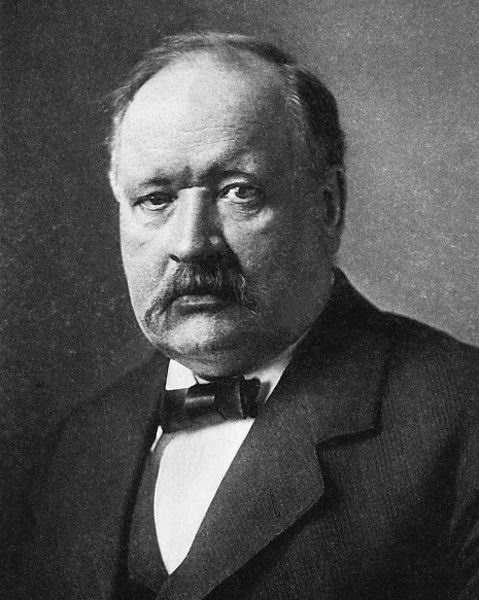
\includegraphics[width=0.22\linewidth]{images/book2/arrhenius.jpg}

{\small 斯万特·阿伦尼乌斯（1859--1927），摄于 1909 年。}
\end{omfigure}

\section{练习}

\begin{exercise}[$\star$]\label{exo:b1:rate-laws:1}
在恒容条件下，对于 \ce{2N2O5 -> 4NO2 + O2}，二氧化氮的
\omterm{def:b1:rate-laws:rate}{生成速率}为 $\qty{2.0e-4}{mol.L^{-1}.s^{-1}}$。求\omterm{def:b1:rate-laws:rate}{反应速率}、氧气的
\omterm{def:b1:rate-laws:rate}{生成速率}以及 \ce{N2O5} 的\omterm{def:b1:rate-laws:rate}{消耗速率}。
\end{exercise}

\begin{exercise}[$\star$]\label{exo:b1:rate-laws:2}
求\omterm{def:b1:rate-laws:order}{总级数}分别为 0、1、2 和 3 时\omterm{def:b1:rate-laws:order}{速率常数}的单位，
浓度以 \unit{mol/L} 计，时间以秒计。
\end{exercise}

\begin{exercise}[$\star$]\label{exo:b1:rate-laws:3}
一级反应 $\mathrm{A} \longrightarrow \mathrm{B}$ 的\omterm{def:b1:rate-laws:order}{速率常数} $k = \qty{3.0e-3}{s^{-1}}$，计算
其\omterm{def:b1:rate-laws:half-life}{半衰期}，以及经过 \qty{10}{min} 后 \ce{A} 的剩余分数。
\end{exercise}

\begin{exercise}[$\star$]\label{exo:b1:rate-laws:4}
某反应物的初始浓度减半时，其\omterm{def:b1:rate-laws:half-life}{半衰期}
加倍。求该反应的级数。若\omterm{def:b1:rate-laws:half-life}{半衰期}减半，情况又如何？
\end{exercise}

\begin{exercise}[$\star\star$]\label{exo:b1:rate-laws:5}
反应物 \ce{A}（$\mathrm{A} \longrightarrow \mathrm{P}$）的浓度经测量：在 $t
= 0$、10、20、30 和 \qty{40}{min} 时，$[\ce{A}] = 0.100$、0.0741、0.0549、
0.0407 和 \qty{0.0301}{mol/L}。确定该反应的级数和
\omterm{def:b1:rate-laws:order}{速率常数}。
\end{exercise}

\begin{exercise}[$\star\star$]\label{exo:b1:rate-laws:6}
对于 $\mathrm{A} + \mathrm{B} \longrightarrow \mathrm{P}$，$v_0 = \qty{2.0e-6}{mol.L^{-1}.s^{-1}}$，当 $[\ce{A}]_0
= [\ce{B}]_0 = \qty{0.010}{mol/L}$ 时；$[\ce{A}]_0$ 加倍时为 \qty{8.0e-6}{}；
$[\ce{B}]_0$ 加倍时为 \qty{4.0e-6}{}。求各
\omterm{def:b1:rate-laws:order}{分级数}、\omterm{def:b1:rate-laws:order}{速率方程}及\omterm{def:b1:rate-laws:order}{速率常数}。
\end{exercise}

\begin{exercise}[$\star\star$]\label{exo:b1:rate-laws:7}
反应 $\mathrm{A} + \mathrm{B} \longrightarrow \mathrm{P}$ 的\omterm{def:b1:rate-laws:order}{速率方程}为 $v = k[\ce{A}][\ce{B}]$。当
$[\ce{B}]_0 = \qty{0.50}{mol/L}$、$[\ce{A}]_0 = \qty{5.0e-3}{mol/L}$ 时，
\ce{A} 按一级动力学消耗，表观\omterm{def:b1:rate-laws:order}{速率常数}为
\qty{0.012}{s^{-1}}。试解释并计算 $k$。
\end{exercise}

\begin{exercise}[$\star\star$]\label{exo:b1:rate-laws:8}
某\omterm{def:b1:rate-laws:order}{速率常数}在 \qty{300}{K} 时为 \qty{1.0e-3}{s^{-1}}，
在 \qty{320}{K} 时为 \qty{5.0e-3}{s^{-1}}。计算\omterm{def:b1:rate-laws:activation-energy}{活化能}及
\qty{310}{K} 时的\omterm{def:b1:rate-laws:order}{速率常数}。
\end{exercise}

\begin{exercise}[$\star\star$]\label{exo:b1:rate-laws:9}
反应 $2\,\mathrm{A} \longrightarrow \mathrm{P}$ 的\omterm{def:b1:rate-laws:order}{速率方程}为 $v = -\frac12\frac{\dd[\ce{A}]}
{\dd t} = k[\ce{A}]^2$，且 $k = \qty{0.50}{L.mol^{-1}.s^{-1}}$。
初始浓度 $[\ce{A}]_0 = \qty{0.020}{mol/L}$，计算\omterm{def:b1:rate-laws:half-life}{半衰期}及
\qty{100}{s} 后的浓度。
\end{exercise}

\begin{exercise}[$\star\star\star$]\label{exo:b1:rate-laws:10}
对一级反应，证明消耗掉分数
$f$ 的反应物所需的时间为 $t_f = -\ln(1 - f)/(ak)$。比较
50\,\%、75\,\%、90\,\% 和 99.9\,\% 所需的时间，以\omterm{def:b1:rate-laws:half-life}{半衰期}计。
\end{exercise}

\begin{exercise}[$\star\star\star$]\label{exo:b1:rate-laws:11}
一种皮肤贴片以恒定速率释放药物，速率为
\qty{0.40}{mg/h}，只要其储药库（初始为 \qty{10}{mg}）未空。
写出剩余药量的规律，给出其级数、\omterm{def:b1:rate-laws:half-life}{半衰期}以及
贴片耗尽的时间。为何零级动力学
适用于药物贴片？
\end{exercise}

\begin{exercise}[$\star\star\star$]\label{exo:b1:rate-laws:12}
证明“温度每升高 10 度，速率加倍”这一规则在
\qty{298.15}{K} 与 \qty{308.15}{K} 之间对应 $E_a \approx
\qty{53}{kJ/mol}$。同一\omterm{def:b1:rate-laws:activation-energy}{活化能}在
\qty{0}{\celsius} 与 \qty{10}{\celsius} 之间给出的因子是多少？
\end{exercise}

\section{问题：药物的有效期}

\begin{problem}[{周末问题——加速稳定性试验：
60\,\textdegree C 下的一级降解、三个温度、
阿伦尼乌斯图以及室温下的有效期}]
\label{pb:b1:rate-laws:1}
为预测片剂的有效期 $t_{90}$（即活性成分降解 10\,\% 所需的时间），
实验室将样品置于高温下保存，
并测定剩余活性成分的百分比。在
\qty{60}{\celsius} 下测得：
\begin{center}
\begin{tabular}{lccccc}
\hline
时间（天） & 0 & 10 & 20 & 30 & 40 \\
剩余活性成分（\%） & 100.0 & 91.4 & 83.5 & 76.3 & 69.8 \\
\hline
\end{tabular}
\end{center}
在 40 和 \qty{50}{\celsius} 时，测得的\omterm{def:b1:rate-laws:order}{速率常数}分别为
\qty{1.27e-3}{d^{-1}} 和 \qty{3.48e-3}{d^{-1}}。取 $R =
\qty{8.314}{J/(mol.K)}$，并取一个月 $= \qty{30.4}{d}$。

\medskip
\noindent\textbf{第一部分——60\,\textdegree C 下的反应级数。}
\begin{enumerate}
  \item 计算每个 10 天区间内的损失量，该反应是否为
        零级反应？
  \item 计算各时刻的 $\ln(\%\text{ 剩余})$。由此能得出什么结论？
  \item 推出\omterm{def:b1:rate-laws:order}{速率常数} $k_{60}$。
  \item 计算 \qty{60}{\celsius} 下的\omterm{def:b1:rate-laws:half-life}{半衰期}。
  \item 在 \qty{60}{\celsius} 下，60 天后剩余的百分比是多少？
  \item 计算 \qty{60}{\celsius} 下的 $t_{90}$。
\end{enumerate}

\medskip
\noindent\textbf{第二部分——保质期与级数。}
\begin{enumerate}[resume]
  \item 证明：对于一级降解，$t_{90} = \ln(10/9)/k$。
  \item 将 $t_{90}$ 表示为\omterm{def:b1:rate-laws:half-life}{半衰期}的分数。
  \item 为什么 $t_{90}$ 与片剂的剂量无关？
  \item 为什么实验室要在高温下测量降解，
        而不在 \qty{25}{\celsius} 下进行？
  \item 若有效成分的降解为二级反应，则效力为两倍的片剂
        保质期会更长还是更短？请说明理由。
\end{enumerate}

\medskip
\noindent\textbf{第三部分——阿伦尼乌斯图。}
\begin{enumerate}[resume]
  \item 对三个温度，列表给出 $1/T$ 与 $\ln k$。
  \item 计算经过 40 和
        \qty{60}{\celsius} 两点的直线斜率。
  \item 由此推出\omterm{def:b1:rate-laws:activation-energy}{活化能}。
  \item 验证 \qty{50}{\celsius} 对应的点落在该直线上。
  \item 计算\omterm{def:b1:rate-laws:activation-energy}{指前因子} $A$。
  \item \omterm{def:b1:rate-laws:rate}{反应速率}在 25 至
        \qty{35}{\celsius} 之间增大了多少倍？与经验规则相比较。
\end{enumerate}

\medskip
\noindent\textbf{第四部分——室温。}
\begin{enumerate}[resume]
  \item 将\omterm{def:b1:rate-laws:order}{速率常数}外推至 \qty{30}{\celsius}。
  \item 计算 \qty{30}{\celsius} 下的 $t_{90}$，单位为月。
  \item 一只盒子在 \qty{60}{\celsius} 的汽车中被遗忘了三天，
        成分损失的比例是多少？
  \item 解释“\qty{25}{\celsius} 以下保存”这一要求。
  \item 将\omterm{def:b1:rate-laws:order}{速率常数}外推至 \qty{25}{\celsius}。
  \item 计算 \qty{25}{\celsius} 下的保质期 $t_{90}$，分别以天和
        月为单位。
\end{enumerate}
\end{problem}
